\documentclass[xcolor=dvipsnames]{beamer}
\useoutertheme{infolines}
\setbeamertemplate{navigation symbols}{}
\setbeamertemplate{items}[ball]
\usepackage{graphicx,multirow,color,xcolor,verbatim,float}
\setbeamertemplate{frametitle}[default][center]
\begin{document}
\title{Efficient methods for identifying mutated driver pathways in cancer}
\author{Bowen Deng}
\institute{Dept. of Prob. and Stat.}
\date{}
\begin{frame}
\maketitle
\end{frame}
\begin{frame}{Generalized framework}
Minimum Penalty Submatrix Problem (MPSP):
\[
\max\sum_{i=1}^m \omega_i p(\sum_{j=1}^n a_{ij}x_j) s.t. \sum_{j=1}^nx_j=k,x_j\in\{0,1\}.
\]
where $a_{ij}(i=1,2,\cdots,m,j=1,2,\cdots,n)\in \{0,1\}$ are elements in mutation matrix A. $\omega_i=1$ for unweighted case and $\omega_i=\frac{1}{\sum_{j=1}^na_{ij}}$ for weighted case.\\
\end{frame}
\section{Simulation Results}
\begin{frame}{Mutation Matrix}
\begin{figure}
\centering
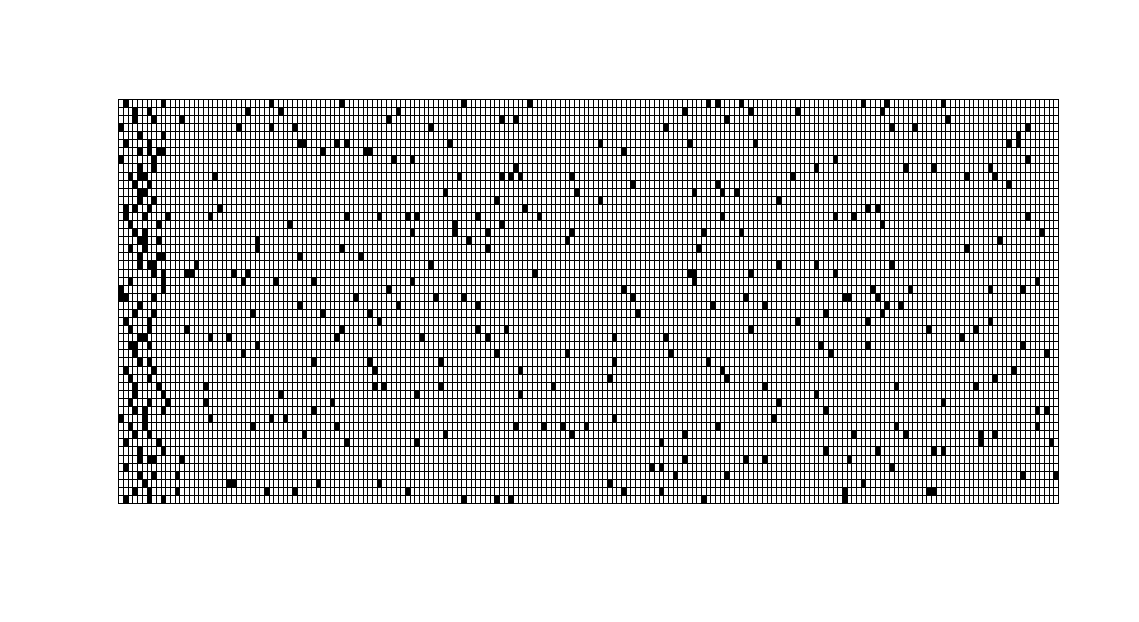
\includegraphics[width=0.8\linewidth]{simulationpic.png}
\end{figure}
We should expect subset of top 10 columns as the driver pathway.\\
\end{frame}
\begin{frame}
\begin{table}
\centering
\begin{tabular}{|c|c|c|c|c|}
\hline
$p_k(x)$&$k$&Weighted&Top10/Total&Penalty/Penalty of top 10\\
\hline
\multirow{6}{*}{$|x-1|$}&\multirow{2}{*}{$\forall$}&No&7/14&2/NA\\
&&Yes&7/14&0.29/NA\\
&\multirow{2}{*}{10}&No&7&4/4\\
&&Yes&8&0.56/0.72\\
&\multirow{2}{*}{5}&No&4/5&16/NA\\
&&Yes&4/5&2.12/NA\\
\hline
\multirow{6}{*}{$\sqrt{|x-1|\cdot k}$}&\multirow{2}{*}{$\forall$}&No&1/1&40/NA\\
&&Yes&1/1&5.88/NA\\
&\multirow{2}{*}{10}&No&8/10&12.65/12.65\\
&&Yes&9/10&2.04/2.30\\
&\multirow{2}{*}{5}&No&5/5&35.78/NA\\
&&Yes&4/5&4.74/NA\\
\hline
\multirow{3}{*}{$\frac{(x-1)^2}{k}$}&$\forall$&No&10/66&0.02/NA\\
&10&No&9/10&0.4/0.4\\
&5&No&4/5&3.2/NA\\
\hline
\end{tabular}
\end{table}
\end{frame}
\section{Application to Biological Datasets}
\begin{frame}{HNSCC}
We have applied our methods to HNSCC (Stransky et al.), which included gene mutation data for $m=74$ patients, $n=4920$ genes.\\
\begin{table}
\centering
\begin{tabular}{r|r}
\hline
$k=2$&$k=3$\\
\hline
\textcolor{red}{SYNE1}, PCLO(50)&LYST, \textcolor{red}{PCLO}, \textcolor{red}{CYNE1}(47)\\
\textcolor{red}{SYNE1}, MUC16(53)&FAT2, FAT1, RYR2(48)\\
USH2A, MUC16(53)&\textcolor{red}{PCLO}, LYST, \textcolor{red}{SYNE1}(47)\\
RIMS2, MUC16(54)&\textcolor{red}{PCLO}, \textcolor{red}{SYNE1}, \textcolor{red}{CDKN2A}(43)\\
\hline
\end{tabular}
\caption{Identified Pathway genes, Penalty of Reference: $k=2$: CDKN2A, SYNE1 is 52; $k=3$: CDKN2A, PCLO, SYNE1 is 43.}
\end{table}
\end{frame}
\begin{frame}
\begin{table}
\begin{tabular}{r}
\hline
\textcolor{red}{PCLO}, \textcolor{red}{ANK2}, \textcolor{red}{CDKN2A}, \textcolor{red}{SYNE1} (39)\\
\textcolor{red}{PCLO}, \textcolor{red}{ANK2}, \textcolor{red}{CDKN2A}, \textcolor{red}{SYNE1} (39)\\
FAT4, \textcolor{red}{CDKN2A}, CSMD3, NOTCH1 (42)\\
\textcolor{red}{PCLO}, \textcolor{red}{ANK2}, \textcolor{red}{CDKN2A}, \textcolor{red}{SYNE1} (39)\\
\hline
\end{tabular}
\caption{Identified Pathway genes, Penalty of Reference: $k=4$: ANK2, CDKN2A, PCLO, SYNE1 is 39}
\end{table}
\end{frame}
\begin{frame}
\begin{table}
\begin{tabular}{r}
\hline
PCLO, ANK2, MYOM2, \textcolor{red}{CDKN2A}, \textcolor{red}{SYNE1} (36)\\
\textcolor{red}{NOTCH1}, FAT4, RYR2, LRP1B, \textcolor{red}{CDKN2A} (36)\\
\textcolor{red}{ANO4}, \textcolor{red}{TP63}, \textcolor{red}{NOTCH1}, \textcolor{red}{SYNE1}, \textcolor{red}{CDKN2A} (35)\\
CASP8, LYST, CUBN, PIK3CA, \textcolor{red}{SYNE1} (39)\\
\hline
\end{tabular}
\caption{Identified Pathway genes, Penalty of Reference: $k=5$: ANO4, CDKN2A, NOTCH1, SYNE1, TP63 is 35}
\end{table}
\end{frame}
\begin{frame}
\begin{table}
\begin{tabular}{r}
\hline
\textcolor{red}{NOTCH1}, \textcolor{red}{NFE2L2}, \textcolor{red}{TP63}, \textcolor{red}{ANO4}, \textcolor{red}{SYNE1}, \textcolor{red}{CDKN2A}(31)\\
\textcolor{red}{ANO4}, UTRN, \textcolor{red}{TP63}, \textcolor{red}{NOTCH1}, \textcolor{red}{SYNE1}, \textcolor{red}{CDKN2A}(32)\\
DOCK1, CUBN, LYST, FMN2, \textcolor{red}{SYNE1}, CASP8(35)\\
\textcolor{red}{NFE2L2}, \textcolor{red}{ANO4}, \textcolor{red}{TP63}, \textcolor{red}{NOTCH1}, \textcolor{red}{CDKN2A}, \textcolor{red}{SYNE1}(31)\\
\hline
\end{tabular}
\caption{Identified Pathway genes, Penalty of Reference: $k=6$: ANO4, CDKN2A, NFE2L2, NOTCH1, SYNE1, TP63 is 31}
\end{table}
\end{frame}
\begin{frame}
\begin{table}
\begin{tabular}{r}
\hline
NFE2L2, TP63, PCDHB11, ANO4, NOTCH1, CDKN2A, SYNE1(28)\\
BRCA2, LRP1B, NCOR1, FAT4, RYR2, NOTCH1, CDKN2A(28)\\
BRCA2, LRP1B, NFE2L2, FAT4, RYR2, NOTCH1, CDKN2A(28)\\
ANK2, UBR4, SLIT3, NOTCH1, SYNE1, PCLO, CDKN2A(30)\\
\hline
\end{tabular}
\caption{Identified Pathway genes, Penalty of Reference: $k=7$: ANO4, CDKN2A, NFE2L2, NOTCH1, SLIT3, SYNE1, TP63 is 28}
\end{table}
\end{frame}
\section{Selection of pathway size}
\begin{frame}
We run each $k$ for fifty times and average the pairwise overlapping length $O(k)$.\\
\[
O(k)=\sum_{1\leqslant i<j\leqslant 50}|A_i\cap A_j|/C_{10}^2
\]
where $A_i$ is the length k pathway detected at the i-th time.\\
We list them in the following table and a higher $O(k)/k$ indicates better stability.\\
\begin{table}
\begin{tabular}{lcc}
$k$&$O(k)$&$O(k)/k$\\
2&0.49&0.24\\
3&0.83& 0.28\\
4&1.31&0.33\\
5&1.68&0.34\\
6&1.86&0.31\\
7&2.92&0.42\\
8&2.94&0.37\\
9&2.76&0.31\\
\end{tabular}
\end{table}
\end{frame}
\begin{frame}
\begin{figure}
\centering
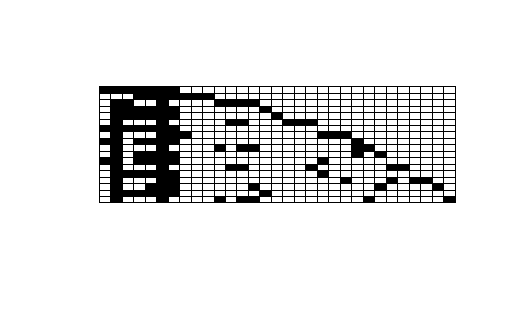
\includegraphics[width=0.6\linewidth]{k7case.png}
\caption{$k=7$: 18 results. Columns for genes. Each row represents one result.}
\end{figure}
We filters out those genes that appear less than four times, and get:\\
GNAS, \textcolor{red}{NOTCH1}, \textcolor{red}{NFE2L2}, \textcolor{red}{TP63}, \textcolor{red}{ANO4}, \textcolor{red}{CDKN2A}, \textcolor{red}{SYNE1}, RYR2, FAT4;\\
for comparison, the driver pathway identified in the paper are:\\
ANO4 CDKN2A NFE2L2 NOTCH1 SLIT3 SYNE1 TP63;\\
ANO4 CDKN2A NFE2L2 NOTCH1 PCDHB11 SYNE1 TP63
\end{frame}
\section{Theoretical Results}
\begin{frame}{Independence Gene Model (IGM)}
Let $A$ be an $m\times n$ mutation matrix so that $\hat{M}$ is the minimal penalty column submatrix of $A$ and $|\hat{M}|=k$.\\
IGM conditions:\\
81. Each gene $g\notin \hat{M}$ is mutated in each patient with probability $p_g\in[p_L,p_U]$, independently of all other events. (Low rate passenger mutation)\\
2. $P(\hat{M})=rm$. (Average row score is constant in respect to $m$)\\
3. $\forall l$, any subset $M\subset \hat{M}$ of cardinality $|M|=l$ satisfies: $P(M)\geqslant \frac{l-d}{k}P(\hat{M})$, for a constant $0\leqslant d<1$. (No dominant submatrix)\\
IGM is a standard assumption for somatic single nucleotide mutations.\\
\end{frame}
\begin{frame}{Technical Conditions}
We have proved that for $m$ sufficiently large, with some technical details, Greedy Algorithm could identify the desired k columns under IGM.\\
Assume $0=p(1)\leqslant p(0)\leqslant p(1)<p(2)<p(3)<\cdots$. $p(\cdot)$ be convex.\\
\[a=-\frac{2r}{k}+p(0)(1-p_U)^2+p(2)p_L^2>0\]
\[b=\frac{-\frac{d+1}{k}r-p_Lp(0)+p_U(p(0)+p(2))\frac{\frac{k-d}{k}r-p(0)}{p(k)-p(0)}}{p(k+1)-p(k)}>0\]
\end{frame}
\begin{frame}{Consistency of Greedy Algorithm}
Denote $M_0=\{r,s\}$ the couple in $\hat{M}$ minimizing $P(M_0)$. If
\[
m\geqslant \frac{(1+\varepsilon/2)\ln{n}p(2)^2}{\min{\{a,b\}}^2},
\]
The greedy algorithm identifies the $m\times k$ column submatrix $\hat{M}$ with minimum penalty $P(\hat{M})$ with probability at least $1-2n^{-\varepsilon}$.\\
\end{frame}
\section{Further Work}
\begin{frame}
Simulation Data: Criteria-Stability\\
Different patient set.\\
Cancer Name For Comparison\\
Fisher's test.\\
Genetic algorithm multiple driver pathways.\\
Network: Combine with expression data.\\
\end{frame}
\end{document}
